\documentclass[11pt,a4paper]{article}

\usepackage[utf8]{inputenc}
\usepackage[T1]{fontenc}
\usepackage[margin=2.4cm]{geometry}
\usepackage{booktabs}
\usepackage{graphicx}
\usepackage{amsmath}
\usepackage[table]{xcolor}
\usepackage[hidelinks]{hyperref}
\usepackage{caption}
\usepackage{enumitem}
\usepackage{tikz}
\usetikzlibrary{arrows.meta,positioning,fit}

\captionsetup{font=small,labelfont=bf}
\setlength{\parskip}{0.4em}
\setlength{\parindent}{0pt}
\graphicspath{{figures/}}

\title{\textbf{Has Peruvian farmland shifted from food crops to export tree crops,\\
and does legal land title cause it?}\\[0.6em]
\large A report on the project to date}
\author{Daniel Ash}
\date{31 August 2026}

\begin{document}
\maketitle

\begin{abstract}
\noindent
This project addresses two questions. First, has farmland in Peru moved from annual crops grown
for the domestic market (rice, maize, beans) to perennial tree crops grown for export (mango,
lime, coffee, banana)? Second, does secure legal title make that move more likely?

The source material is the archive of Peru's land-titling programme, which records for
approximately one million parcels both the parcel boundary and the crop growing on it. It
records this only once, mostly between 1997 and 2006. Satellite imagery is available for every
year from 1996. The intended design was to treat the archive as training labels, fit a
classifier, apply it to every year, and read the change from the resulting series.

The classifier works. The year-by-year series does not, for reasons that can be stated
precisely. Three direct measurements of the change were substituted. All three agree that the
perennial share rose by approximately ten percentage points between about 1999 and 2012. None
finds that legal title accounts for it: the best-powered estimate has titled parcels shifting
slightly less than untitled ones, and a formal causal estimate on national data is a tight null
between $-1.3$ and $+1.0$ percentage points.

One methodological finding runs through the report and reversed several earlier conclusions.
Cross-validation that holds out nearby land systematically overstates how well a model performs
in a region it has never seen. Every input and every model selected on cross-validation alone
required re-examination.
\end{abstract}

\tableofcontents
\newpage

%======================================================================
\section{Summary of results}

\begin{table}[htbp]
\centering
\small
\caption{Every line of work and its outcome.}
\label{tab:scoreboard}
\begin{tabular}{@{}p{5.0cm}p{4.2cm}p{6.0cm}@{}}
\toprule
\textbf{Attempted} & \textbf{Outcome} & \textbf{Reason} \\
\midrule
Distinguish 12 individual crops from imagery
& Fails
& Annual crops share a single seasonal curve at 30\,m resolution \\[0.4em]

Distinguish perennial from annual from bare ground
& Works, 0.68 macro-F1 on held-out data
& Year-round canopy is visible; crop identity is not \\[0.4em]

Extend to the whole country
& Works, and is more stable than one department alone
& 14 departments, 946{,}872 parcels \\[0.4em]

Apply the classifier to every year, 1996--2023, for a per-parcel history
& Fails
& A classifier that is correct 55--59\,\% of the time cannot support a 25-year series per parcel \\[0.4em]

Aggregate that history into 5-year windows
& Fails
& The comparison group drifts seven times further than the signal, in the opposite direction \\[0.4em]

Correct the drift (recalibration, sensor harmonisation, density matching)
& Four routes closed by measurement
& The sensor difference depends on land cover, so no single linear correction removes it \\[0.4em]

Photo-interpret recent high-resolution imagery
& Works, 865 parcels labelled
& Supplies the only accuracy measured in the period of interest \\[0.4em]

Compare the 1999 declaration with the 2012 agricultural census
& Works, 63{,}766 parcels
& Two independent declarations of the same land, with no imagery and no classifier \\[0.4em]

Place 1999, 2012 and 2025 on one axis and split by tenure
& Consistent in level; uninformative on tenure
& The 2025 estimate is $-1.0$ points if abandoned woody vegetation is excluded and $+13.2$ if it counts as perennial, with intervals near $\pm 17$ \\[0.4em]

Estimate the causal effect of legal title
& A tight null
& $-0.11$ points, 95\,\% interval $[-1.26, +1.04]$ \\
\bottomrule
\end{tabular}
\end{table}

Three results merit separate statement.

\textbf{1. The perennial share rose by approximately ten percentage points.} Between the titling
declaration (median year 1999) and the 2012 agricultural census, the share of parcels declaring a
perennial crop rose from 16.5\,\% to 26.4\,\% nationally, and from 21.0\,\% to 33.5\,\% measured
by land area. The flow is strongly asymmetric: 7{,}158 parcels moved from annual to perennial
against 1{,}832 in the reverse direction.

\textbf{2. Legal title does not account for it.} Titled parcels rose 9.2 points and untitled
parcels 11.3 points. Measured by area the difference disappears ($+10.7$ against $+11.0$). A
formal causal estimate on 14{,}625 parcels and 15 years of imagery returns $-0.11$ points, with
an interval containing zero under every assumption tested.

\textbf{3. Most land declared as annual cropland in 1999 is not currently cropped.} Read directly
from 865 photo-interpreted parcels, 57.9\,\% of parcels that declared an annual crop are farmable
ground with nothing growing on them, and 2.9\,\% read as perennial. This is a national average
and does not describe Piura, where 86.7\,\% of such parcels still carry annual crops.

%======================================================================
\section{Data}

\subsection{Sources}

Four archives were used. None was documented, and establishing the contents of each file and the
relationships between them formed a substantial part of the work.

\begin{table}[htbp]
\centering
\small
\caption{The raw sources.}
\label{tab:sources}
\begin{tabular}{@{}p{3.2cm}rp{9.6cm}@{}}
\toprule
\textbf{Source} & \textbf{Size} & \textbf{Description} \\
\midrule
Crop registry (BD SSET)
& 5.6\,M rows
& One row per parcel-crop declaration made to the land-titling programme. Carries the crop as
free text, the parcel area, and the parcel's legal registration status at declaration. It is not
a census: only parcels enrolled in the programme appear. \\[0.4em]

Cadastral bridge
& 1.87\,M rows
& The only file carrying both the registry's parcel key and the map's parcel key. Everything
depends on it. It also carries a second observation of legal status, dated around 2011--12. \\[0.4em]

Parcel maps
& 2.9\,M polygons
& Parcel boundaries, from 24 shapefiles. \\[0.4em]

2012 agricultural census
& 17.75\,M rows
& An independent national survey of what each farmer grows, covering all 25 departments. It
carries no parcel key, so it links to the rest only through the farmer's name. \\
\bottomrule
\end{tabular}
\end{table}

\subsection{Linkage}

Figure~\ref{fig:chain} shows the two linkages. The first uses real keys on both joins and yields
the training set. The second uses the farmer's name and yields the paired comparison of
Section~\ref{sec:census}.

\begin{figure}[htbp]
\centering
\resizebox{\textwidth}{!}{%
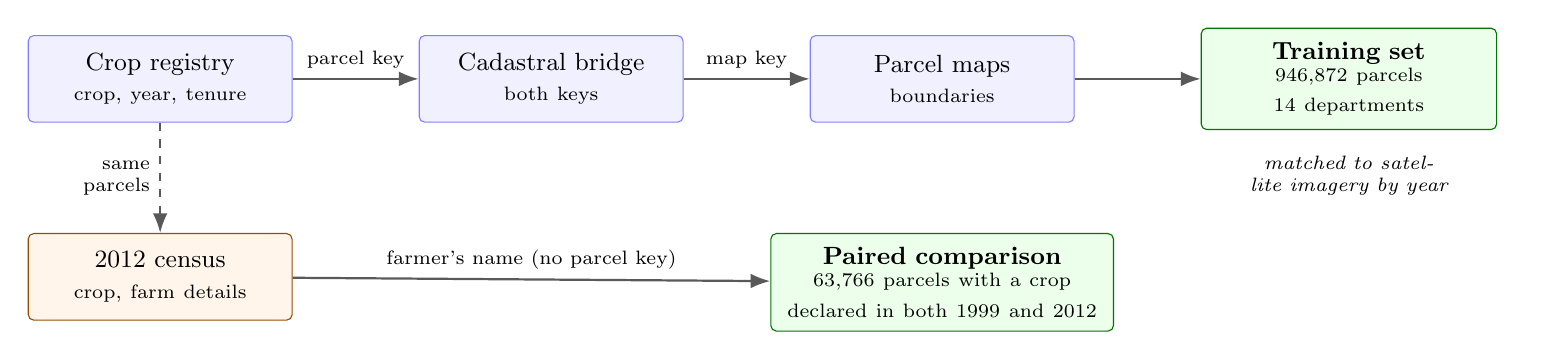
\begin{tikzpicture}[
  node distance=6mm,
  box/.style={draw, rounded corners=2pt, align=center, font=\small, inner sep=5pt,
              minimum height=11mm, text width=30mm},
  srcbox/.style={box, fill=blue!6, draw=blue!50},
  resbox/.style={box, fill=green!8, draw=green!45!black, text width=34mm},
  cenbox/.style={box, fill=orange!8, draw=orange!60!black},
  arr/.style={-{Latex[length=2.5mm]}, thick, draw=black!65}
]
\node[srcbox] (sset) {Crop registry\\\scriptsize crop, year, tenure};
\node[srcbox, right=16mm of sset] (bridge) {Cadastral bridge\\\scriptsize both keys};
\node[srcbox, right=16mm of bridge] (poly) {Parcel maps\\\scriptsize boundaries};
\node[resbox, right=16mm of poly] (train) {\textbf{Training set}\\\scriptsize 946{,}872 parcels\\\scriptsize 14 departments};

\draw[arr] (sset) -- node[above, font=\scriptsize] {parcel key} (bridge);
\draw[arr] (bridge) -- node[above, font=\scriptsize] {map key} (poly);
\draw[arr] (poly) -- (train);

\node[cenbox, below=14mm of sset] (cen) {2012 census\\\scriptsize crop, farm details};
\node[resbox, below=14mm of poly, text width=40mm] (pair) {\textbf{Paired comparison}\\\scriptsize 63{,}766 parcels with a crop\\\scriptsize declared in both 1999 and 2012};

\draw[arr] (cen) -- node[above, font=\scriptsize] {farmer's name (no parcel key)} (pair);
\draw[arr, dashed] (sset) -- node[left, font=\scriptsize, align=right] {same\\parcels} (cen.north);

\node[font=\scriptsize\itshape, below=2mm of train, text width=44mm, align=center]
  {matched to satellite imagery by year};
\end{tikzpicture}}
\caption{The two linkages. The upper chain uses real keys on both joins and forms the training
set. The lower chain matches only on the farmer's name, so it identifies the person reliably and
the individual parcel only approximately. Its results are therefore reported by link quality and
reweighted before any national claim is made.}
\label{fig:chain}
\end{figure}

\subsection{Coverage, and why its limits are permanent}

The cadastral bridge exists for only 15 departments, and one of those (Callao) yields nothing
usable. The bridge is mandatory, since no other file carries both keys, so the project covers
\textbf{14 departments}. Approximately 653{,}000 parcels in eight further departments have
boundaries but no route to a crop label; two departments have crop labels but no boundaries.

The consequence is that \textbf{no labels exist for the sierra or the Amazon}, and none can be
produced from this source. Every accuracy figure in this report describes coastal and
lower-altitude farmland.

Two further properties bind everything downstream. Registration dates are unreliable: a single
stub date accounts for about 35\,\% of Piura's rows, so the year is a titling date rather than a
verified growing season. And crops are grown in blocks. About 86\,\% of neighbouring parcels in
Piura share a crop, against 46\,\% under random placement, so any train/test split must hold out
whole areas of land rather than random parcels.

%======================================================================
\section{Classification}

\subsection{The three models}

Three models were compared throughout, on identical parcels, identical folds and identical
inputs. All read a single parcel's own satellite record; none uses any neighbouring parcel.

The imagery is reduced to \textbf{11 channels} per observation date: the six surface-reflectance
bands (blue, green, red, near infrared, and two shortwave infrared) plus five derived indices
(NDVI, EVI, NDWI, NDMI and BSI) measuring greenness, moisture and exposed bare soil.

\begin{table}[htbp]
\centering
\small
\caption{The three models and what each one reads.}
\label{tab:models}
\begin{tabular}{@{}p{2.4cm}p{5.2cm}p{6.8cm}@{}}
\toprule
\textbf{Model} & \textbf{What it is} & \textbf{Input} \\
\midrule
\textbf{LightGBM}
& Gradient-boosted decision trees. A sequence of shallow trees, each correcting the errors of
those before it.
& About 135 summary numbers per parcel-year: for each of the 11 channels, the median, mean,
standard deviation, minimum, maximum, quartiles, seasonal amplitude, linear slope and a
first-order harmonic fit, plus a few parcel attributes such as area. Dates are discarded once
summarised. \\[0.4em]

\textbf{LTAE}
& Lightweight Temporal Attention Encoder. A small neural network that learns which dates in the
year carry the information and weights them accordingly.
& The dated series itself: up to 64 observation dates $\times$ 11 channels, with the day of year
attached to each and a mask marking cloud-obscured dates. Nothing is summarised in advance. \\[0.4em]

\textbf{rules}
& A registered control: a hand-written decision rule of depth two, using three greenness
thresholds.
& Three of the summary columns. Included to establish an honest floor, not as a competitor. \\
\bottomrule
\end{tabular}
\end{table}

\subsubsection{F1 score}
F1 score measures a model’s balance between precision and recall, using their harmonic mean; a high F1 means the model performs well on both.
Macro-F1 calculates the F1 score separately for each class and then averages them equally, making it useful for imbalanced datasets because each class has the same influence regardless of its size.

\subsection{Twelve crops: not separable}

The first design asked directly which of twelve crops was growing. It does not work. On 49{,}648
parcels the best model reached 0.427 macro-F1, where guessing rice for every parcel gives 0.425
accuracy.

Figure~\ref{fig:profiles12} shows why. Cotton, maize, beans, wheat and zarandaja produce
essentially the same greenness curve: a peak between March and May, senescent by August. Only
rice, which is flooded and therefore spectrally distinctive, and coffee, which holds an evergreen
canopy, separate cleanly.

\begin{figure}[htbp]
\centering
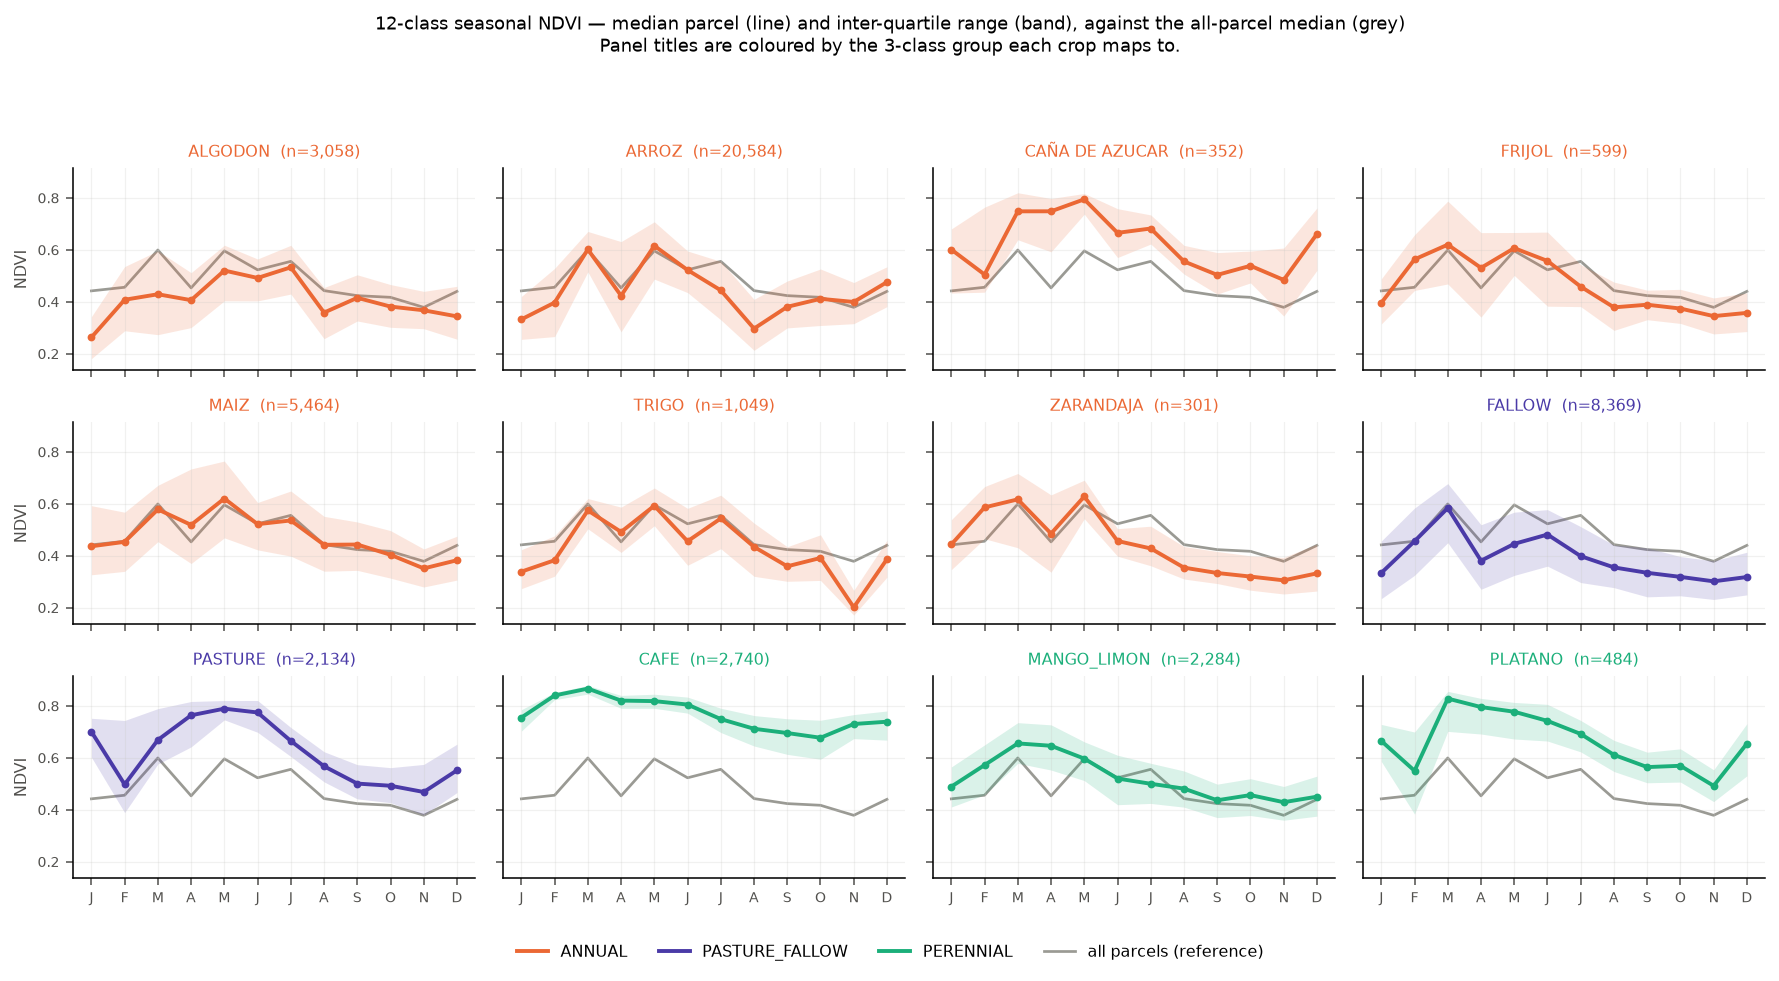
\includegraphics[width=\textwidth]{profiles_12class_ndvi.png}
\caption{Seasonal greenness for each of the twelve crops, against the all-parcel median in grey.
The five annual crops in the upper rows are nearly indistinguishable from one another and from
the median. The three perennial crops in the bottom row sit clearly above it all year.}
\label{fig:profiles12}
\end{figure}

\begin{table}[htbp]
\centering
\small
\caption{Per-class results for the twelve-crop model.}
\label{tab:12class}
\begin{tabular}{@{}lrr@{\hspace{2em}}lrr@{}}
\toprule
\textbf{Crop} & \textbf{F1} & \textbf{n} & \textbf{Crop} & \textbf{F1} & \textbf{n} \\
\midrule
Rice     & 0.751 & 16{,}446 & Cotton      & 0.376 & 2{,}855 \\
Coffee   & 0.698 & 2{,}322  & Maize       & 0.228 & 4{,}175 \\
Wheat    & 0.666 & 661      & Banana      & 0.197 & 448 \\
Mango / lime & 0.529 & 1{,}435 & Sugar cane & 0.147 & 339 \\
Fallow   & 0.512 & 7{,}224  & Beans       & 0.114 & 501 \\
\bottomrule
\end{tabular}
\end{table}

\subsection{Three land states: separable}

The distinction the imagery supports is not which crop, but whether the parcel holds canopy all
year. That is also the distinction the research question requires, since perennial approximates
export and annual approximates domestic.

Regrouping into three classes --- perennial, annual, and pasture or fallow --- gives a classifier
that works. On a held-out test set of 9{,}671 Piura parcels it reaches \textbf{0.681 macro-F1} at
0.748 accuracy, against 0.671 for the majority guess. The test score exceeded the
cross-validation score of 0.647, which is the reassuring direction: residual leakage in the
spatial splits did not inflate the estimate.

\begin{figure}[htbp]
\centering
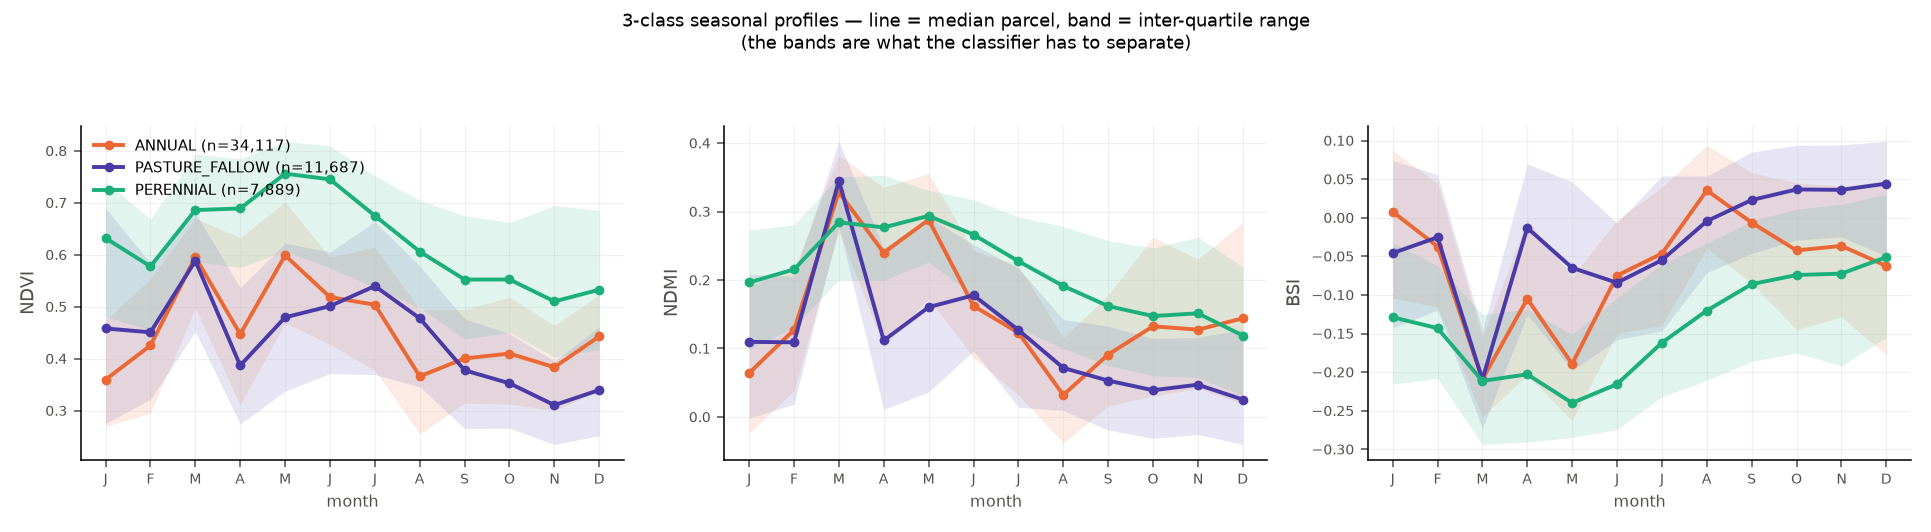
\includegraphics[width=\textwidth]{profiles_3class.png}
\caption{The three-class problem. Perennial parcels stay green and moist and expose less bare
soil; annual parcels peak and senesce; pasture and fallow sit between. The shaded bands are the
interquartile range of each class. They overlap, which is why the classifier reaches 0.68 rather
than 0.95.}
\label{fig:profiles3}
\end{figure}

\begin{table}[htbp]
\centering
\small
\caption{The three-class classifier on its held-out test set, and against the best available
off-the-shelf land-cover product.}
\label{tab:3class}
\begin{tabular}{@{}lrrr@{}}
\toprule
& \textbf{macro-F1} & \textbf{accuracy} & \textbf{coverage} \\
\midrule
LightGBM (Piura, held-out test, n = 9{,}671) & \textbf{0.681} & 0.748 & 100\,\% \\
Majority guess & --- & 0.671 & --- \\
MapBiomas Peru, best configuration & 0.385 & 0.580 & 90\,\% \\
\midrule
\multicolumn{4}{@{}l}{\emph{Per-class F1:} annual 0.833 \quad perennial 0.769 \quad pasture/fallow 0.440}\\
\bottomrule
\end{tabular}
\end{table}

The MapBiomas comparison requires an honest reading. MapBiomas Peru loses because \emph{it has no
perennial class in Piura at all}: its perennial crop, coffee, citrus and pasture codes never
appear in the department, and 63\,\% of our parcels fall into a single mixed-use bucket that
combines orchards, coffee and fallow. This is a structural gap rather than a contest won. The
useful conclusion is the positive one: a parcel-level model is necessary here precisely because
the off-the-shelf product does not resolve the distinction the question depends on.

LightGBM was selected over LTAE at this stage under a pre-registered tie-break: LTAE led by
0.0027 macro-F1, inside the 0.02 threshold, at roughly one hundred times the computational cost.

\subsection{National extension}

Rebuilding on all 14 departments gives 946{,}872 linked parcels, of which 726{,}808 resolve to
one of the three land states. Accuracy falls very slightly; stability improves considerably.

\begin{table}[htbp]
\centering
\small
\caption{One department against fourteen.}
\label{tab:national}
\begin{tabular}{@{}lrr@{}}
\toprule
& \textbf{Piura} & \textbf{All 14 departments} \\
\midrule
Linked parcels & 66{,}352 & 946{,}872 \\
Label years carrying more than 5\,\% of the data & 2 & 8 \\
Cross-validation macro-F1 & 0.648 & 0.628 \\
Variation across folds & $\pm$0.036 & $\pm$0.013 \\
Perennial F1 & 0.685 & 0.655 \\
Pasture / fallow F1 & 0.485 & 0.606 \\
\bottomrule
\end{tabular}
\end{table}

One caution attaches to every share computed from this sample. Small departments were
deliberately over-sampled so that each would carry enough parcels to learn from, and the small
departments are the coastal, perennial ones. The sample is 20.2\,\% perennial against a
population value of 9.9\,\%, so any statement about how much land is in a given state must be
reweighted to the population.

%======================================================================
\section{Evaluation}
\label{sec:evaluation}

This section contains the finding that reversed the most conclusions.

\subsection{Four tests rather than one}

Because crops grow in blocks, held-out parcels were selected as whole 5\,km blocks of land with a
buffer stripped from the training side. That is stricter than standard practice and still
insufficient. Once the project covered 14 departments, a larger unit could be held out: an entire
department. Four tests were then applied to every candidate: hold out a 5\,km block inside a
department already seen; hold out a whole department; hold out a whole year; hold out a
department and a year together.

\subsection{Latitude resembles information and is not}

Parcel latitude was among LightGBM's inputs. In Peru, latitude is nearly a label for the climate
zone, so it resembles agricultural information.

\begin{table}[htbp]
\centering
\small
\caption{The value of parcel latitude as a LightGBM input, under four tests.}
\label{tab:latitude}
\begin{tabular}{@{}lr@{}}
\toprule
\textbf{Test} & \textbf{Change in macro-F1} \\
\midrule
Held-out 5\,km block, same department & $+0.048$ \\
Held-out year & $+0.047$ \\
\textbf{Held-out department} & $\mathbf{-0.060}$ \\
Held-out department and year & $-0.005$ \\
\bottomrule
\end{tabular}
\end{table}

Latitude's contribution reverses sign as soon as the held-out unit is a place, and 12 of the 14
departments score better without it. It was not encoding climate; it was serving as a lookup
table for departments already memorised. Holding out a year does not detect this, because a year
held out leaves the geography unchanged, so a time-invariant input remains exactly as exploitable
as in ordinary cross-validation.

Two consequences follow. The gap between predicting a nearby block and predicting an unseen
department is about 0.09 macro-F1, and a single-department project has no means of observing it.
And a claim carried for months --- that Piura is among the hardest departments to predict ---
proved to be an artefact of this one input: Piura ranks 13th of 14 with latitude and 6th without.

\subsection{The same pattern in a model architecture}

\begin{figure}[htbp]
\centering
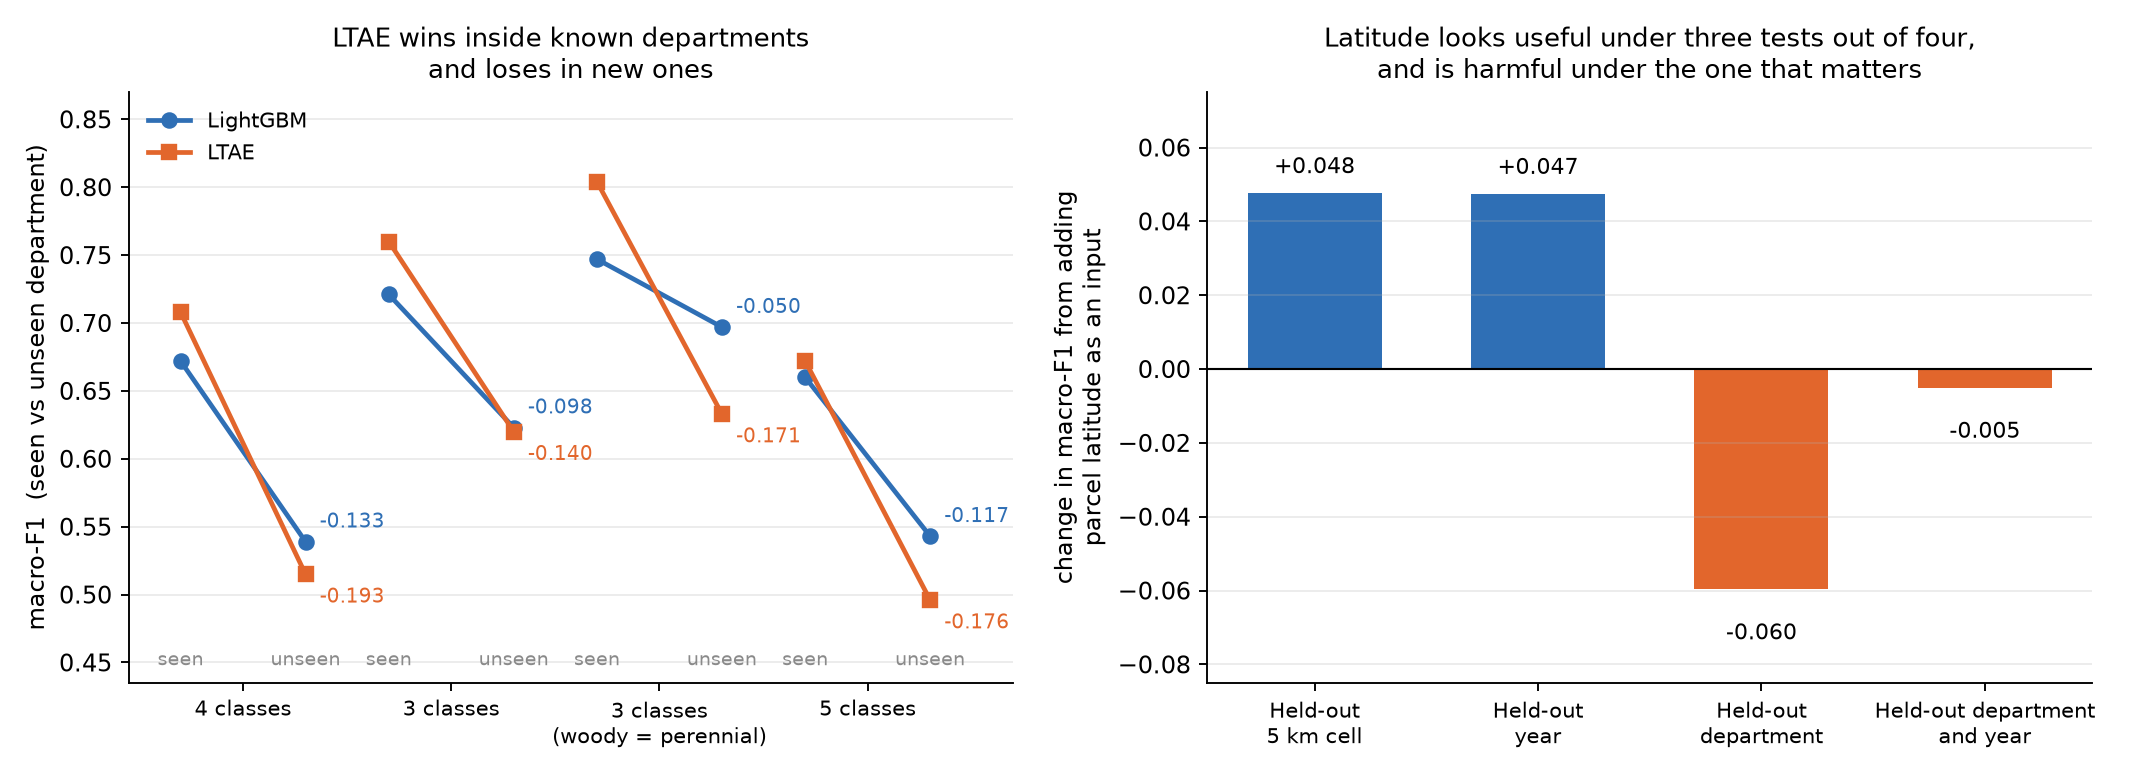
\includegraphics[width=\textwidth]{cv_vs_lodo.png}
\caption{Left: LTAE beats LightGBM on all four label groupings when the held-out land lies inside
a known department, and loses on all four when a whole department is held out, falling 1.4 to 3.4
times further. Right: the same pattern for a single input, parcel latitude.}
\label{fig:cvlodo}
\end{figure}

Tested on the same parcels, folds and features, LTAE wins cross-validation in all eight arms by
0.013 to 0.068, and loses the held-out-department test in all four label groupings. Its
additional skill does not leave the training departments. This is the latitude failure again,
produced by an architecture rather than an input. LightGBM was carried forward.

The rule adopted for the remainder of the project: \textbf{no input or model is selected on
cross-validation alone, and all four tests are reported.}

\subsection{A trap in the headline metric}

Macro-F1 averages the per-class score with equal weight, which makes it incomparable across
different numbers of classes: the score of a model that does nothing rises as classes are
removed. Collapsing the labels to perennial-or-not raises macro-F1 from 0.672 to 0.715 and raises
the do-nothing floor from 0.171 to 0.467.

\begin{table}[htbp]
\centering
\small
\caption{The two-class collapse produces the highest raw score and the least skill. Skill
rescales the score so that 0 is always guessing the largest class and 1 is perfect.}
\label{tab:floor}
\begin{tabular}{@{}lrrrrr@{}}
\toprule
\textbf{Label grouping} & \textbf{Classes} & \textbf{Floor} & \textbf{macro-F1} & \textbf{Skill}
& \textbf{Perennial F1} \\
\midrule
5 classes & 5 & 0.124 & 0.660 & 0.612 & 0.523 \\
4 classes & 4 & 0.171 & 0.672 & 0.604 & 0.471 \\
3 classes, woody counted as perennial & 3 & 0.228 & 0.747 & 0.672 & 0.768 \\
\rowcolor{red!7} 2 classes, perennial or not & 2 & 0.467 & \textbf{0.715} & \textbf{0.465} & 0.509 \\
\bottomrule
\end{tabular}
\end{table}

Collapsing four classes into two gains $+0.028$ on the perennial class and collapsing three into
two gains $+0.004$, while discarding four interpretable outputs. A binary answer should be taken
by summing the multi-class probabilities instead.

The same experiment settled something more useful. The two-class arms differ only in which side
non-crop woody vegetation is placed on, and that single choice moves perennial F1 from 0.620 to
0.810 --- six times the effect of collapsing the label space. The binding difficulty is not the
number of classes but that an orchard and a stand of riverside scrub look alike from orbit.

%======================================================================
\section{Why a year-by-year history is not available}

The original design was to apply the classifier to every year from 1996 to 2023 and read the
trend from the result. Two checks were registered before the attempt: predictions should degrade
gracefully when applied to years distant from the training years, and a parcel's predicted
history should not alternate implausibly. The second check failed in every arm.

\subsection{Predicted histories are dominated by noise}

A perennial orchard does not become an annual field and revert. The flicker rate counts parcels
whose predicted class changes implausibly often; the criterion set in advance was 0.15.

\begin{table}[htbp]
\centering
\small
\caption{Flicker on the national 25-year panel, 114{,}125 parcel-years per arm. All three fail.}
\label{tab:flicker}
\begin{tabular}{@{}lrrr@{}}
\toprule
\textbf{Model} & \textbf{Time-invariant inputs} & \textbf{Flicker (criterion 0.15)} & \textbf{Accuracy} \\
\midrule
LightGBM, with latitude & 3 & 0.517 & 0.586 \\
LightGBM, without latitude & 2 & 0.744 & 0.544 \\
LTAE, no static inputs at all & 0 & 0.980 & 0.581 \\
\bottomrule
\end{tabular}
\end{table}

\begin{figure}[htbp]
\centering
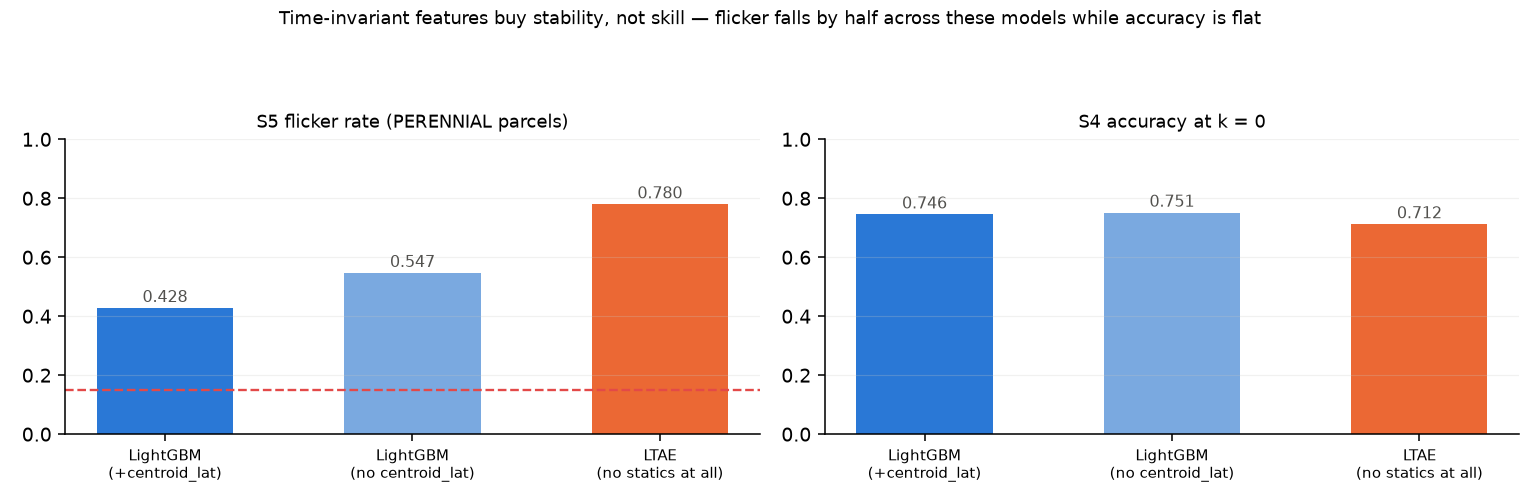
\includegraphics[width=\textwidth]{flicker_vs_statics.png}
\caption{The same result on the Piura panel. Flicker roughly doubles as time-invariant inputs are
removed, while accuracy is flat. Time-invariant inputs purchase the appearance of stability, not
the ability to be correct.}
\label{fig:flicker}
\end{figure}

The ordering in Table~\ref{tab:flicker} was predicted before the runs and reproduced
exactly. A model that always returns the same answer for a parcel appears stable and has learned
nothing about that parcel's history, so the flicker measurement is itself gameable and the honest
reading is the worst one rather than the best.

Three explanations are ruled out by measurement. Prediction quality does not degrade with
distance in time on the national panel, so the training years are not the cause. Satellite
coverage exceeds 93\,\% in all 25 years, so missing imagery is not the cause. The failure
worsens when the architecture is changed, so the model is not the cause.

What remains is arithmetic. Errors in different years are close to independent, so a series of 25
predictions from a classifier that is correct 55--59\,\% of the time is dominated by
classification noise. \textbf{No per-parcel trajectory, transition series or area trend was
produced from this panel, and none should be.} The code that would produce them is written,
tested and deliberately unrun.

\subsection{The 1998 El Niño makes the baseline years unusable}

A second, independent obstacle concerns the baseline. The panel's first years, 1996--98, include
the 1997--98 El Niño flood. A model trained on 1999 and 2000 and applied to 1998 returns
perennial recall of \textbf{0.000}, against 0.361 on a control year.

\begin{figure}[htbp]
\centering
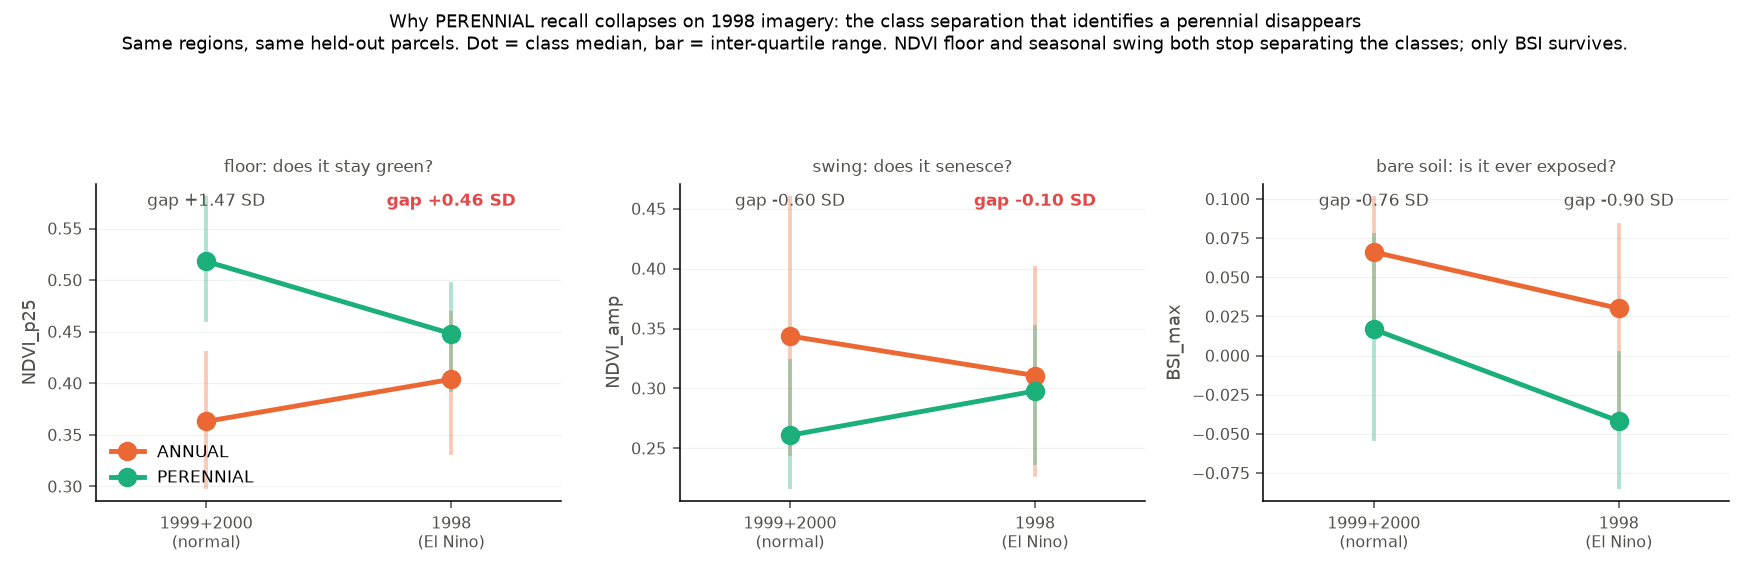
\includegraphics[width=\textwidth]{elnino_mechanism.png}
\caption{The mechanism. A perennial parcel is identified not by an absolute greenness level but
by the gap between it and annual parcels on the same measure. The flood closed that gap from both
sides: perennials lost canopy while flooded annual ground stayed green. A threshold learned in
normal years then falls inside both distributions. Only the bare-soil measure survives.}
\label{fig:elnino}
\end{figure}

Since 1996--98 are the baseline years, the perennial baseline is near zero for reasons unrelated
to the land, and any rise measured from it would be an artefact. Restricting training to 1999
onwards repairs the temporal-degradation check but not the flicker check.

\subsection{Aggregation and correction do not repair it}

Aggregating predictions to five-year windows does fix the instability: 82\,\% of parcels never
change state. It does not fix the estimate. Parcels already perennial at declaration form the
comparison group and should stay flat; instead their predicted perennial share drifts down by
0.044 to 0.103 per decade while the group of interest rises by 0.018. The comparison group moves
seven times further than the signal, in the opposite direction.

Part of the mechanism was identified. Landsat observation density falls from about 24 to about 13
clear observations per parcel-year as one satellite is retired and another develops a scanning
fault, and as evidence thins, predicted probabilities move toward the base rate for both classes.
At the level of a share that is indistinguishable from conversion. It accounts for up to 29\,\%
of the drift.

Four corrections were tried and measured shut. The most informative failure was admitting the
newer Landsat sensor, attempted twice, including once with coefficients refitted on 27{,}573
same-day observations of the same parcels by both satellites. It cannot work for a structural
reason: the sensor difference depends on land cover --- 0.070 greenness units on perennial
parcels against 0.045 on pasture --- and no single linear correction applied to all parcels can
remove a difference between them.

%======================================================================
\section{Direct measurement of the change}
\label{sec:census}

With the year-by-year route closed, the change was measured three other ways. None requires a
working annual series, and two require no classifier at all.

\subsection{Photo-interpretation of recent imagery}

Every accuracy figure above is measured in 1997--2006, whereas the research question concerns
2019--2023. A labelling campaign was therefore built: 1{,}112 parcels drawn from a national
eligible universe of 614{,}876, each presented as a high-resolution image chip together with its
Sentinel-2 record, and labelled by hand into five categories.

\begin{table}[htbp]
\centering
\small
\caption{The labelling campaign against its pre-registered acceptance criteria.}
\label{tab:gates}
\begin{tabular}{@{}p{4.6cm}p{3.0cm}p{2.3cm}p{5.0cm}@{}}
\toprule
\textbf{Check} & \textbf{Criterion} & \textbf{Result} & \textbf{Reading} \\
\midrule
Share of parcels the labeller could not call
& below 25\,\%
& \textbf{13.9\,\% pass}
& At 1.2\,m resolution, 86\,\% of parcels are callable. This was the principal unknown. \\[0.4em]

Labels per department
& at least 35
& \textbf{48 pass}
& All 14 departments clear it, so a department can be held out. \\[0.4em]

Agreement between two passes over the same parcels
& at least 0.75
& \textbf{not}\newline\textbf{measured}
& The overlap batch has not been returned. This is the campaign's principal outstanding gap. \\
\bottomrule
\end{tabular}
\end{table}

1{,}012 labels were returned and 865 are usable. Sentinel-2 supplies a median of 19 to 113 clear
observations per parcel-year by department, against 13 to 24 in the Landsat archive.

Trained on these labels, LightGBM reaches \textbf{0.672 macro-F1} on held-out blocks of land and
\textbf{0.539} on a held-out department across four classes; on a three-class reading, 0.747 and
0.697. These are the only accuracy figures measured on imagery from the period of interest.

One limitation attaches to every number in this section. There was a single labeller, and the
check that would quantify that labeller's consistency has not been run, so all figures below
inherit an unmeasured amount of labelling noise.

\subsection{What the labels show without a classifier}

The campaign's most useful output requires no model. Cross-tabulating what the titling programme
recorded in 1996--2006 against what a person observes on current imagery gives
Figure~\ref{fig:transition}.

\begin{figure}[htbp]
\centering
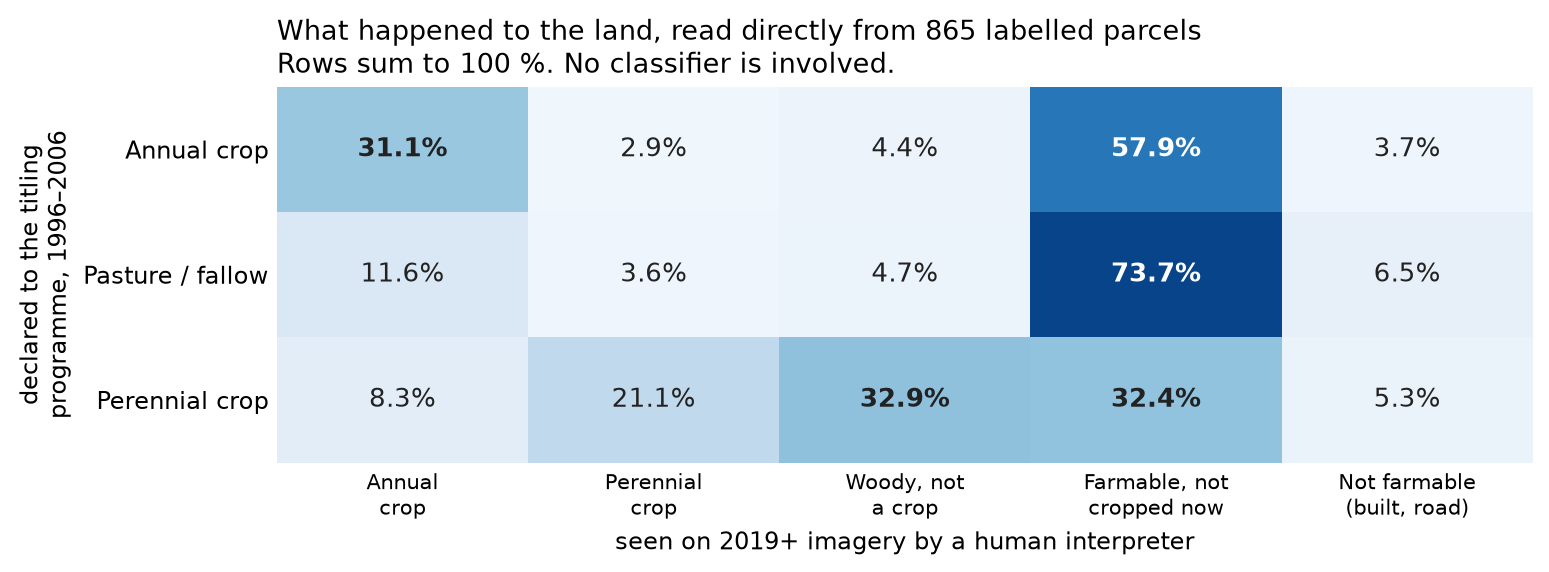
\includegraphics[width=\textwidth]{transition_matrix.png}
\caption{Declared land use in 1996--2006 against observed land use in 2019 or later, on 865
parcels, weighted to the national population. The 95\,\% interval on the 2.9\,\% cell runs from 0
to 5.9.}
\label{fig:transition}
\end{figure}

Three readings follow, in order of importance.

\textbf{The expected shift is not visible here.} Of parcels that declared an annual crop, 2.9\,\%
read as perennial, indistinguishable from zero. What they overwhelmingly read as is farmable
ground not currently cropped: 57.9\,\%. Parcels that declared pasture or fallow behave the same
way.

\textbf{This is a national average describing nowhere in particular.} Restricted to Piura,
86.7\,\% of declared-annual parcels still carry annual crops and only 6.7\,\% are uncropped.
Piura's irrigated coastal valleys remain in cultivation; the national figure is carried by other
departments. Piura contributes 65 parcels, so the contrast is indicative rather than precise.

\textbf{The bottom row is a warning about the whole exercise.} Only 21.1\,\% of parcels that
declared a perennial crop still read as perennial. A third read as woody vegetation that is not a
crop, and a further third as uncropped. Whether a parcel is an abandoned orchard or riverside
scrub that was never a crop is the hardest call in the labelling scheme, it carries a third of
the perennial sample, and its reliability is precisely what has not been measured.

\subsection{The 2012 census as the earlier observation}

The strongest measurement in the project uses no imagery and no classifier. The 2012 agricultural
census is an independent second declaration of what is growing on some of the same parcels, which
converts a one-observation design into a paired one.

\begin{table}[htbp]
\centering
\small
\caption{Perennial share at the titling declaration (median 1999) and at the 2012 census, on the
same parcels. Percentage points.}
\label{tab:census}
\begin{tabular}{@{}lrrrr@{}}
\toprule
\textbf{Measure} & \textbf{n} & \textbf{$\sim$1999} & \textbf{2012} & \textbf{Change} \\
\midrule
Piura only, by parcel & 8{,}669 & 28.2\,\% & 40.7\,\% & $+12.5 \pm 0.9$ \\
National, by parcel, as linked & 63{,}766 & 24.6\,\% & 33.0\,\% & $+8.4 \pm 0.3$ \\
\textbf{National, by parcel, reweighted} & 63{,}766 & 16.5\,\% & 26.4\,\% & $\mathbf{+9.9 \pm 0.3}$ \\
National, by cadastral area, reweighted & 63{,}766 & 21.0\,\% & 33.5\,\% & $+12.5$ \\
\bottomrule
\end{tabular}
\end{table}

The gross flows matter more than the net change: \textbf{7{,}158 parcels moved from annual to
perennial against 1{,}832 in the reverse direction}, a ratio of nearly four to one. Perennial
declarations are also persistent, at 92.9\,\%, which is what a tree crop should do and an annual
rotation should not. Conversion occurred on the larger parcels: those that switched had a median
area of 0.85\,ha against 0.38\,ha for those that remained annual, which is why the change is
larger by area than by parcel count.

Three limitations bind the comparison.

\emph{The link is by farmer name.} Which of a farmer's parcels a census row refers to is
uncertain. By link quality the change is $+8.0$ points for high-confidence links, $+8.0$ for
medium, and $+15.6$ for the 4\,\% classed as low. High and medium agree to the decimal over
92\,\% of the sample, which is what makes the result credible; the low tier behaves as an
unreliable link should.

\emph{The linked sample is not random.} It requires a name on both sides and district agreement,
and the parcels satisfying that are the larger, better-documented ones. The linked panel is
16.6\,\% perennial against a population value of 9.9\,\%, so reweighting on department and
declared class is required. Reweighting raises the estimate from $+8.4$ to $+9.9$, so composition
was damping the change rather than creating it.

\emph{The two instruments do not share a class space.} The titling programme records a land state
and has an explicit resting category; the census asks which crop is grown, so a fallow parcel
contributes no row. Crossing them raw makes pasture and fallow appear to collapse from 30.8\,\%
to 6.3\,\%, which is the instrument rather than the land. Every figure above is restricted to
parcels with a crop recorded on both sides.

\subsection{The three measurements together}

\begin{figure}[htbp]
\centering
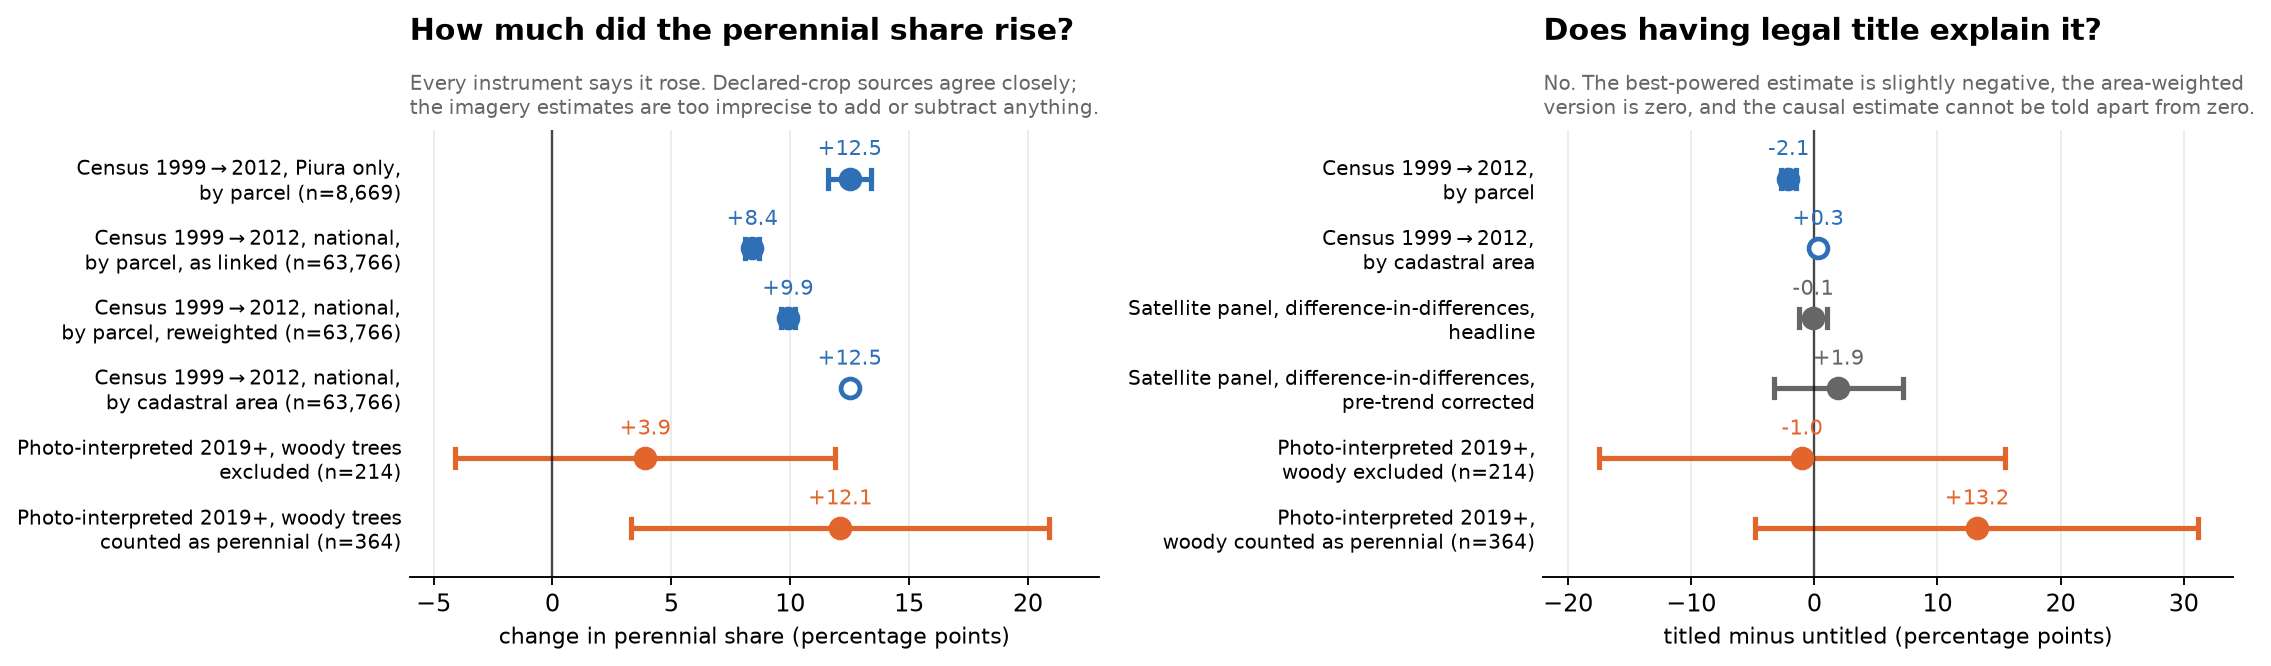
\includegraphics[width=\textwidth]{shift_and_tenure.png}
\caption{Left: every instrument agrees the perennial share rose, and the two declared-crop
sources agree closely on the magnitude. The imagery estimates are consistent with them and far
too imprecise to add anything. Right: no instrument finds that legal title accounts for the rise.}
\label{fig:forest}
\end{figure}

The photo-interpreted arm gives $+3.9 \pm 8.0$ points with woody vegetation excluded and
$+12.1 \pm 8.8$ with it counted as perennial. Both are consistent with the census estimate of
$+9.9$, and neither can distinguish itself from it or from zero. The treatment of one ambiguous
class moves the answer by 8 points, which exceeds the effect being measured. This is
Section~\ref{sec:evaluation}'s conclusion again: the binding constraint is that boundary, not the
sample size.

%======================================================================
\section{The effect of legal title}

\subsection{Design}

Two dated observations of a parcel's legal status already exist: the status recorded at
declaration (1997--2006) and the cadastre's own status with its transaction date (about
2011--12). This yields 1{,}780{,}580 parcels with two dated observations, of which 8.6\,\% moved
from unregistered to registered --- sufficient for a difference-in-differences design with no new
data collection.

\begin{table}[htbp]
\centering
\small
\caption{Sample construction. The final treated group is every qualifying parcel in Peru, not a
sample of them.}
\label{tab:did}
\begin{tabular}{@{}p{9.6cm}r@{}}
\toprule
\textbf{Restriction} & \textbf{Parcels} \\
\midrule
Declared an annual crop, legal status resolved & 363{,}529 \\
Both observations carry a date & 254{,}209 \\
Cadastre observation falls after the declaration & 254{,}033 \\
The pre-period lies entirely before the parcel's own declaration & 80{,}868 \\
After defining the comparison group & 32{,}399 \\
\midrule
\textbf{Drawn: 6{,}559 treated (all that exist) and 8{,}066 comparison} & \textbf{14{,}625} \\
\bottomrule
\end{tabular}
\end{table}

Fifteen years of imagery were extracted for these parcels: 211{,}567 parcel-years and 63.6
million pixel observations. LightGBM supplies the outcome at both dates, drift included; the
design relies on that drift being common to both groups and cancelling. The analysis was
registered in writing before the extraction was funded, including a placebo test that the code
path forces to be estimated first.

\subsection{Result: a tight null}

\begin{figure}[htbp]
\centering
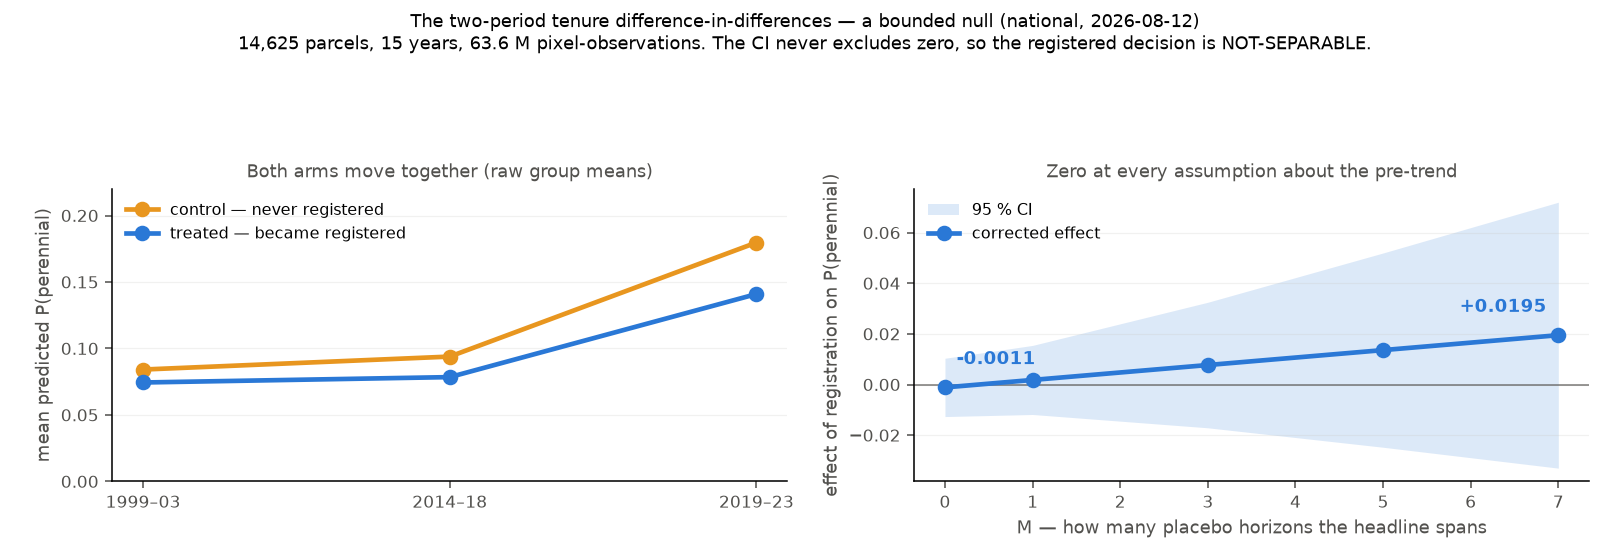
\includegraphics[width=\textwidth]{did_result.png}
\caption{Left: both groups move together. Right: the estimated effect of becoming registered
under increasingly severe assumptions about how much pre-existing trend to subtract. The interval
contains zero throughout.}
\label{fig:did}
\end{figure}

The headline estimate is $\mathbf{-0.0011}$ with a 95\,\% interval of $[-0.0126, +0.0104]$: legal
registration moves the predicted perennial probability by less than 1.3 percentage points in
either direction, measured on the entire national population of qualifying parcels.

A placebo test on a period before any registration returns $-0.0029$, so a correction was applied
for the possibility that the groups were already diverging. The correction widens the interval
from $\pm 1.3$ to $\pm 5.3$ points rather than revealing a large effect beneath a trend. The
conclusion is unchanged at every correction strength tested. Discounting for the fact that only
57.3\,\% of perennial land carries export crops gives $+1.1$ points, interval $[-1.9, +4.1]$.

The sample cannot be enlarged: 6{,}559 treated parcels is every qualifying parcel in Peru.
Requiring an earlier cohort, so that two clean pre-periods exist, leaves 380 treated parcels.

\subsection{The census reaches the same conclusion independently}

The paired census comparison of Section~\ref{sec:census} can be split by legal status at
declaration, using no imagery and no classifier.

\begin{table}[htbp]
\centering
\small
\caption{Change in perennial share, 1999 to 2012, by legal status at declaration.
Post-stratified to the national population.}
\label{tab:tenure}
\begin{tabular}{@{}lrrrr@{}}
\toprule
\textbf{Status at declaration} & \textbf{n} & \textbf{$\sim$1999} & \textbf{2012} & \textbf{Change} \\
\midrule
Registered & 40{,}161 & 15.1\,\% & 24.2\,\% & $+9.2$ \\
Not registered & 23{,}605 & 19.2\,\% & 30.5\,\% & $+11.3$ \\
\midrule
\textbf{Difference} & 63{,}766 & $-4.1$ & $-6.3$ & $\mathbf{-2.1 \pm 0.6}$ \\
\midrule
\multicolumn{4}{@{}l}{\emph{The same difference measured by land area}} & $+0.3$ \\
\bottomrule
\end{tabular}
\end{table}

\begin{figure}[htbp]
\centering
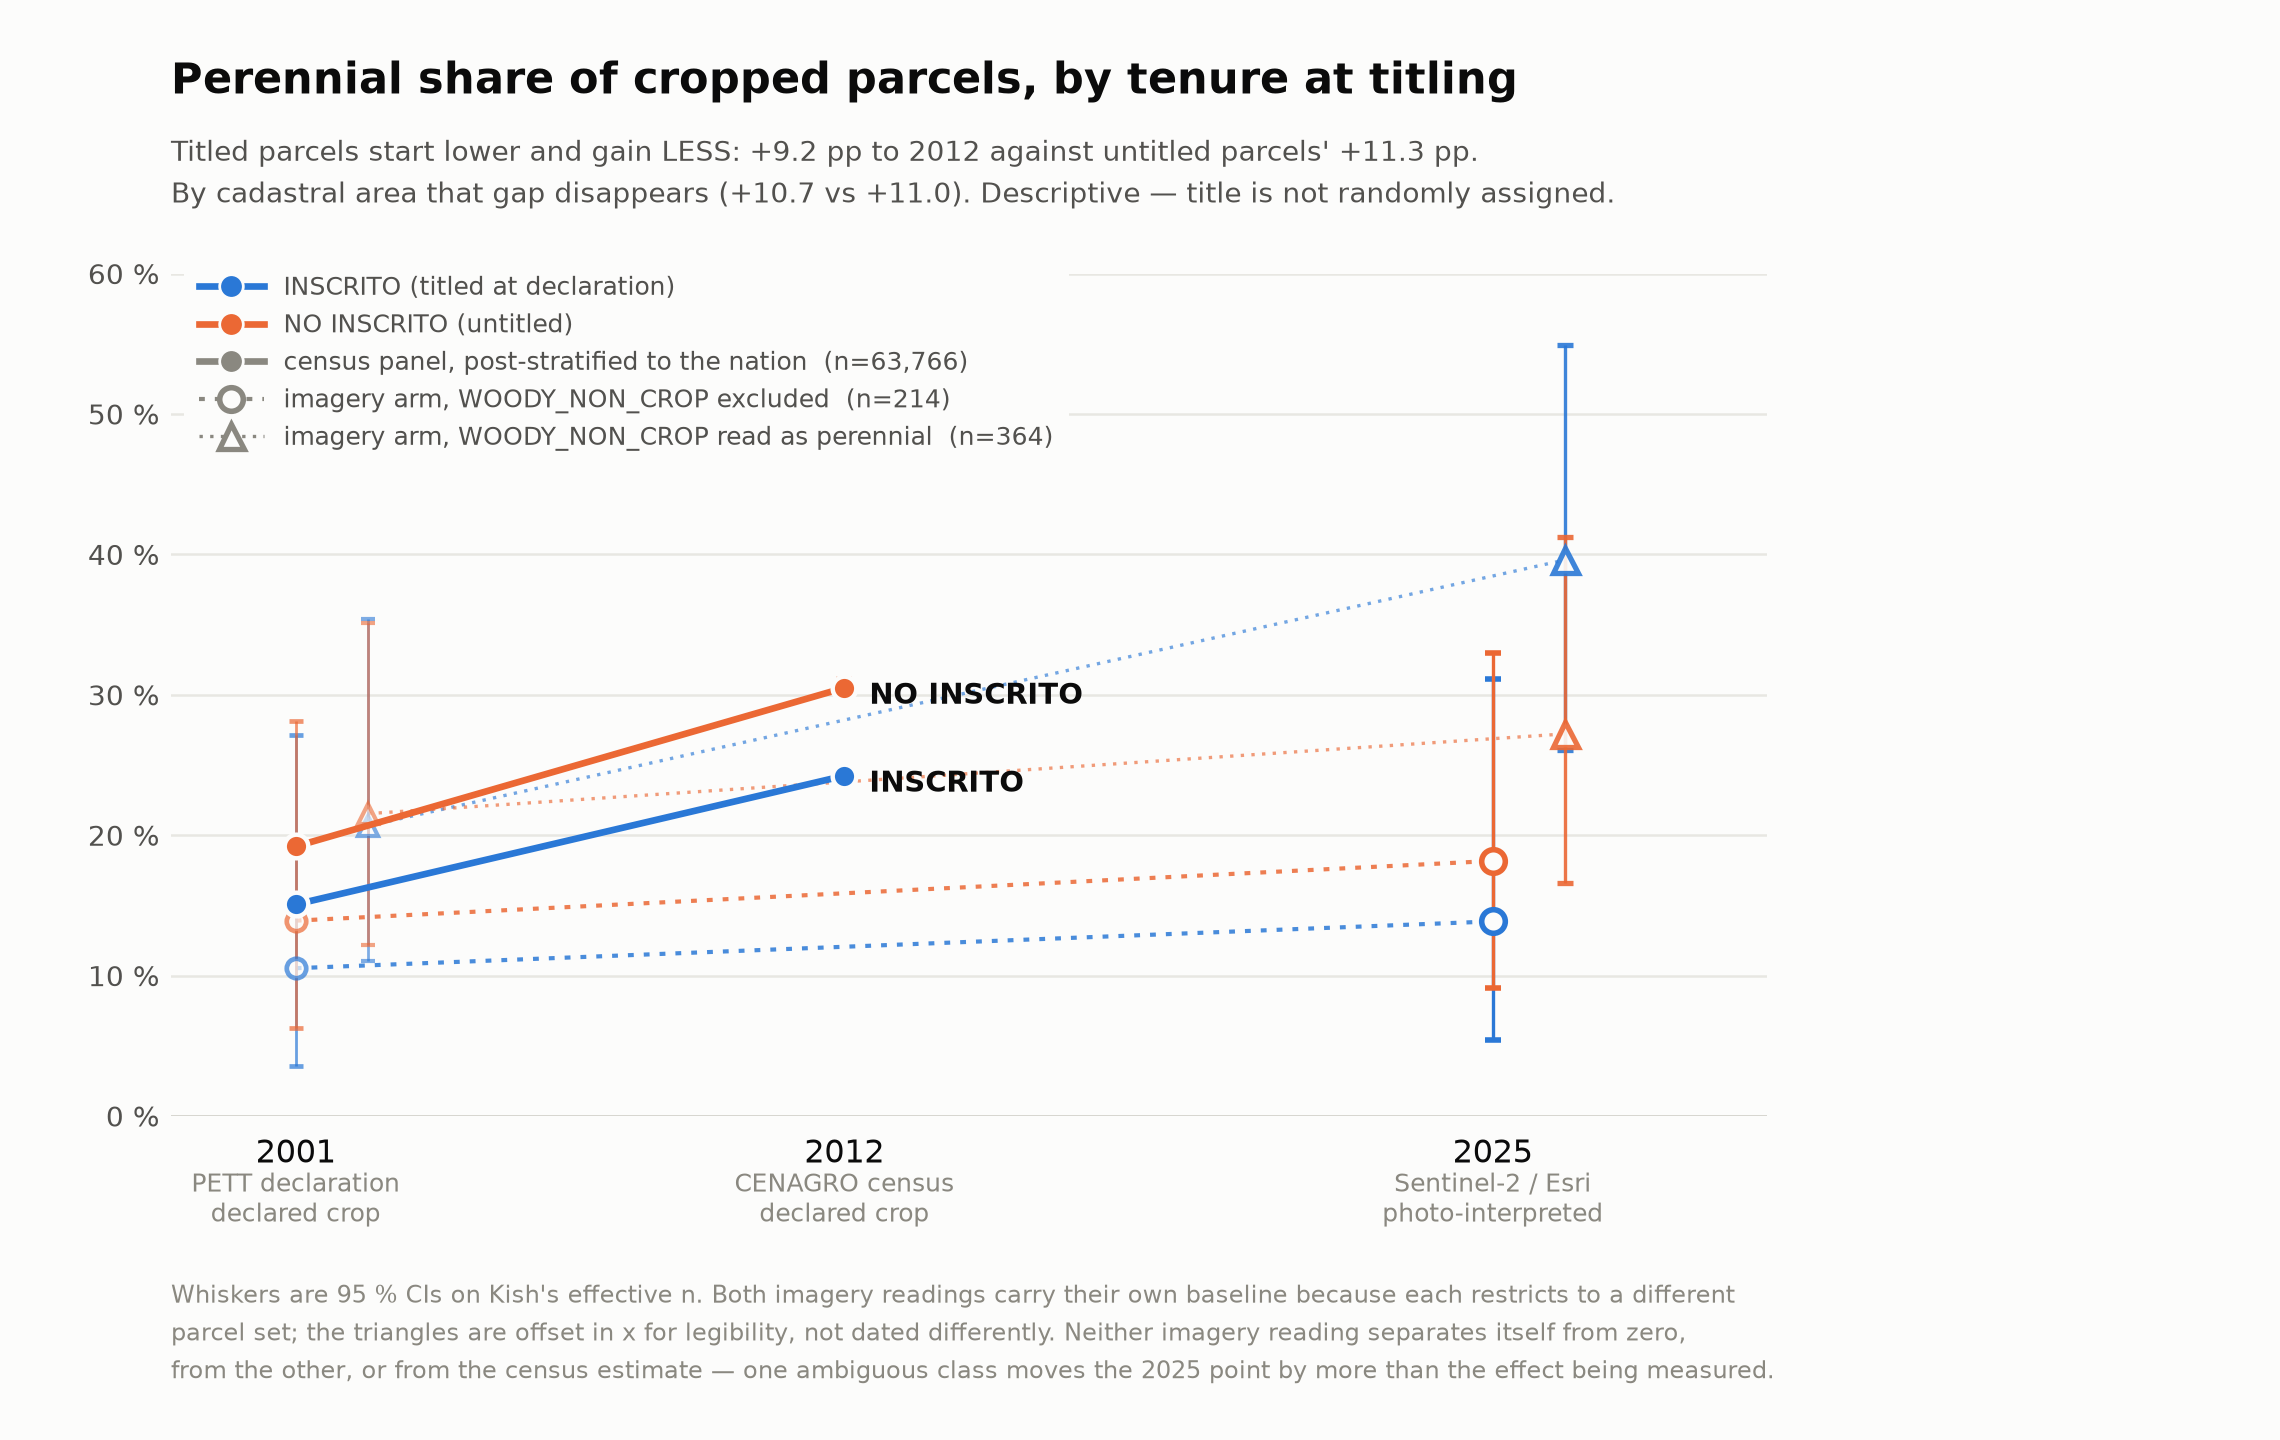
\includegraphics[width=0.95\textwidth]{perennial_over_time_by_tenure.png}
\caption{The three observations of the same quantity. The solid lines are the census panel; the
2025 points come from a different frame with a different restriction, so each is drawn from its
own baseline rather than continued from the census line. Joining them would invent a trend
neither source measured.}
\label{fig:tenure}
\end{figure}

Titled parcels shifted less, by about 2 points on a base of about 10. Measured by land area the
gap disappears: $+10.7$ against $+11.0$. A difference that reverses sign between counting parcels
and counting hectares is not an effect but a difference in parcel size between the groups.

The 2025 photo-interpreted arm cannot adjudicate this. Excluding woody vegetation it gives
$-1.0 \pm 16.5$ points; counting woody vegetation as perennial it gives $+13.2 \pm 18.0$. Two
readings of one ambiguous class, opposite in sign, with intervals an order of magnitude wider
than the census estimate.

Two further cautions. The sign varies by department --- 9 of 14 negative, 5 positive, the
positives all small southern or sierra departments --- so the national figure averages a
distribution straddling zero. And title is not randomly assigned: registered parcels began 4.1
points lower on perennials, precisely the kind of pre-existing difference the correction in
Figure~\ref{fig:did} exists to discipline.

\subsection{What would change this answer}

One limitation binds every tenure number in this report. Legal status is last observed in about
2011--12, the outcome runs to 2023, and Peru's titling programme continued operating. An unknown
share of the comparison group was titled afterwards, unobserved, which biases any real effect
toward zero. A positive finding here would therefore have been an underestimate, and \textbf{this
result is partly attributable to that contamination and is not evidence that titling has no
effect}. Bounding it requires a third dated observation of legal status, which does not exist in
these archives. Reopening the question requires a dated registration event from a different
source, not more of this one.

A related finding is easily misread. The simple cross-sectional association --- whether
registered parcels are more perennial than unregistered ones --- turns out, at the baseline year,
to equal the classifier's own false-positive-rate gap between the two groups, measured
independently from a different direction. The baseline association is a property of the
instrument rather than of the land.

%======================================================================
\section{Climate covariates}

Almost every input tested in this project either helped only within known departments or helped
nowhere. One exception was found. Adding the parcel's mean temperature and mean annual rainfall
as two further inputs improved the recent-imagery classifier on both tests.

\begin{table}[htbp]
\centering
\small
\caption{Climate inputs on the recent-imagery classifier, 704 parcels, four classes. The final
row of each block is a control: parcel latitude and longitude in place of the two climate values,
matching them in number and in smoothness over space but carrying no agricultural content.}
\label{tab:climate}
\begin{tabular}{@{}llrrrr@{}}
\toprule
\textbf{Model} & \textbf{Inputs added} & \textbf{Held-out} & \textbf{Held-out} & \textbf{Perennial} & \textbf{Departments} \\
 & & \textbf{block} & \textbf{department} & \textbf{F1} & \textbf{improved} \\
\midrule
LightGBM & none & 0.672 & 0.539 & 0.471 & --- \\
LightGBM & temperature & 0.695 & 0.568 & 0.564 & 11 of 14 \\
LightGBM & rainfall & 0.691 & 0.561 & 0.536 & 8 of 14 \\
\textbf{LightGBM} & \textbf{both} & \textbf{0.701} & \textbf{0.577} & \textbf{0.574} & \textbf{12 of 14} \\
LightGBM & \emph{latitude/longitude} & 0.696 & 0.553 & 0.546 & --- \\
\midrule
LTAE & none & 0.708 & 0.515 & 0.592 & --- \\
LTAE & both & 0.716 & 0.543 & 0.594 & --- \\
LTAE & \emph{latitude/longitude} & 0.708 & 0.553 & 0.577 & --- \\
\bottomrule
\end{tabular}
\end{table}

The control row makes the table readable. Climate is a smooth function of location, so ``climate
helps'' and ``the model memorised where it is'' predict the same improvement. Substituting two
coordinates for the two climate values, holding everything else fixed, separates them. LightGBM
obtains 2.7 times more out-of-department improvement from climate than from coordinates, and the
improvement is concentrated in the perennial class, whose viability is physically set by
temperature and water. LTAE obtains the same improvement from both, so for LTAE the climate input
is location memorisation by another route, and it was not adopted.

The general rule, now applied throughout: \textbf{where an input is a smooth function of
something the model must not memorise, the decisive comparison is not the input against nothing,
but the input against a same-shaped substitute carrying only the property of concern.}

Two constraints attach. Climate values alone recover the department at 0.676 accuracy against a
0.091 baseline, so the memorisation route remains open and is merely outweighed here; it would
not stay outweighed on a different set of departments. And these are long-run normals, hence
time-invariant, so they must never enter a year-by-year model, where they would manufacture
exactly the false stability of Table~\ref{tab:flicker}.

%======================================================================
\section{Limitations}

\begin{enumerate}[leftmargin=1.6em,itemsep=3pt]
\item \textbf{Geography.} 14 departments, all coastal or lower-altitude. No sierra or Amazon
labels exist in these archives and none can be produced from them.

\item \textbf{The labels are declarations, not observations.} The titling programme recorded what
a farmer stated was growing, once, at an unreliable date. The 2012 census is a second
declaration, not an audit.

\item \textbf{Almost every accuracy figure is measured in 1997--2006.} Only the recent-imagery
figures fall in the period of interest, and those rest on 865 labels from a single labeller whose
consistency is unmeasured.

\item \textbf{The census link is by farmer name.} It identifies the person well and the parcel
only approximately, and the linked sample over-represents larger, better-documented parcels.
Reweighting is applied but cannot address selection within a category.

\item \textbf{Legal status is last observed in 2011--12} while the outcome runs to 2023. Later
titling in the comparison group is unobserved and biases any real effect toward zero.

\item \textbf{One ambiguous class carries a third of the perennial sample.} Whether abandoned
woody vegetation counts as perennial moves the 2025 estimates by 8 points on the level and by 14
points on the tenure split, both exceeding the effect being measured.

\item \textbf{Some held-out test sets are spent.} The Piura test set was used twice and is no
longer a clean estimate for model selection. The national and recent-imagery test sets remain
unspent.
\end{enumerate}

%======================================================================
\section{Conclusions}

\textbf{The substantive question.} Peruvian farmland covered by these archives did shift toward
perennial crops: approximately 10 percentage points of parcels and 12 of land area between 1999
and 2012, with annual-to-perennial conversion outnumbering the reverse by nearly four to one and
concentrated on larger parcels. Three sources agree within their uncertainty. The picture from
2019 onwards is not simply more orchards, however. On the national sample, most land that
declared an annual crop in 1999 is now farmable ground with nothing growing on it, and that
finding does not hold in Piura, the department on which every earlier stage of the project was
built.

\textbf{The causal question.} Legal title does not appear to drive the shift. The formal estimate
is a tight null, the independent census comparison points slightly the other way, and its
area-weighted version is zero. This is a bounded null rather than a demonstration of no effect:
unobserved later titling in the comparison group biases the estimate toward zero, and the
population of parcels capable of answering the question is exhausted.

\textbf{Method.} The finding that generalises beyond Peru is that cross-validation on spatially
blocked data still overstates performance in unseen regions, and does so invisibly unless a whole
region can be held out. It caught an input (latitude), an architecture (LTAE) and an entire class
of features (anything time-invariant, in a year-by-year model). In each case the decisive
quantity was not the one normally reported. One further rule earned its place the same way: a new
input should be scored against a same-shaped substitute rather than against nothing.

\subsection*{Next steps}

\begin{enumerate}[leftmargin=1.6em,itemsep=2pt]
\item \textbf{Measure the labelling noise.} One hundred parcels re-labelled after an interval
would give the campaign its own consistency estimate. Every recent-imagery figure currently
inherits an unmeasured noise floor, and this is now a better use of 100 labels than additional
training data, since the learning curve has flattened.
\item \textbf{Decide whether to spend the held-out test set.} 201 parcels, of which 161 are
labelled, would supply the only clean out-of-sample estimate for the period of interest, at
approximately $\pm$7 points. It can be spent once, on one pre-declared model.
\item \textbf{Do not reopen the tenure question with this data.} It requires a dated registration
event from another archive.
\end{enumerate}

%======================================================================
\appendix
\section{Work built, tested and deliberately unrun}

Six pieces of analysis code are complete and unit-tested and have never been run on real data,
because the check that would license their output failed. They are retained, and retained unrun,
so that the reason remains on the record.

\begin{table}[htbp]
\centering
\small
\begin{tabular}{@{}p{6.0cm}p{8.4cm}@{}}
\toprule
\textbf{Intended output} & \textbf{Reason it is not run} \\
\midrule
Per-parcel transition series & Predicted histories are dominated by classification noise \\
Corrected area and share estimates over time & As above \\
Comparison against national agricultural statistics & As above \\
Sensor correction between Landsat generations & Measured to be worse than no correction \\
Locally refitted sensor correction & The difference depends on land cover; no linear map removes it \\
Larger tenure difference-in-differences & The qualifying population is exhausted \\
\bottomrule
\end{tabular}
\end{table}

\section{Software}

Python 3.11, managed with \texttt{uv}. Approximately 77 modules under
\texttt{src/crop\_classifier/} cover label construction, spatially blocked splitting, Google Earth
Engine extraction, feature assembly, the three model families of Table~\ref{tab:models}, and the
analysis for each section above. 29 test files pin the linkage logic, the split logic, the
extraction robustness and each analysis. Everything runs through a single command-line entry
point.

Imagery is Landsat 5 and 7 surface reflectance for the historical work and Sentinel-2 for the
recent-imagery work, both via Google Earth Engine. The raw archives (about 20\,GB) and all model
outputs are held locally and are not in version control.

\end{document}
